El propósito de este capítulo es definir el modelo estándar rápidamente, enfocándonos en el sector electrodébil, y mostrar que ha sobrevivido muchas pruebas experimentales. Esto hace del modelo estándar una teoría excelente, válida en un amplio rango de energías y el límite al cual otras teorías `más allá del modelo estándar' deberían aproximarse a `bajas energías'.

\section[\hspace{-0.14in}Introducción]{Introducción}

A finales de la década de 1970, el Modelo Estándar (ME) de la física de partículas, creado por Weinberg, Salam y Glashow, comenzó a consolidarse como la teoría básica de la materia. Aquí los constituyentes fundamentales son partículas de spin $1/2$ y son llamados \textit{quarks} y \textit{leptones}. Estas interacciones entre partículas es mediada por otras partículas de spin $0$ (el bosón de Higgs) y $1$ (fotones, gluones y los bosones W y Z) \cite{Weinberg:1967tq}. 


Hasta una década antes del ME, se pensaba que los protones, neutrones, piones, kaones y otras partículas que interactuaban fuertemente (hadrones) eran elementales. Sin embargo, el consenso que surgió más adelante fue que los hadrones estaban compuestos de bloques más básicos llamados quarks y se mantenían unidos mediante el intercambio de gluones \cite{hoddeson1992rise}.

En la figura \ref{SMparticles} podemos ver los seis sabores $f$ para los quarks, es decir, $f= u$ (arriba), $d$ (abajo), $c$ (encantado), $s$ (extraño), $t$  (cima) y $b$ (fondo) en rosado, los seis leptones: el electrón (e), el muón ($\mu$) y el tau ($\tau$), más sus neutrinos asociados ($\nu_e, \nu_{\mu}, \nu_{\tau}$) en verde, y los portadores de fuerza: el fotón ($\gamma$), el gluón (g) y los bosones Z y W en anaranjado. Finalmente, en amarillo tenemos el bosón de Higgs el cual está separado de los otros bosones por no ser un bosón de gauge. Esto último quiere decir que no está asociado al grupo de gauge del ME, $SU(3)_C \times SU(2)_L \times U(1)_Y$, donde $C,L,Y$ representan color, quiralidad izquierda e hipercarga, respectivamente. 

\begin{figure}[!h]
\centering
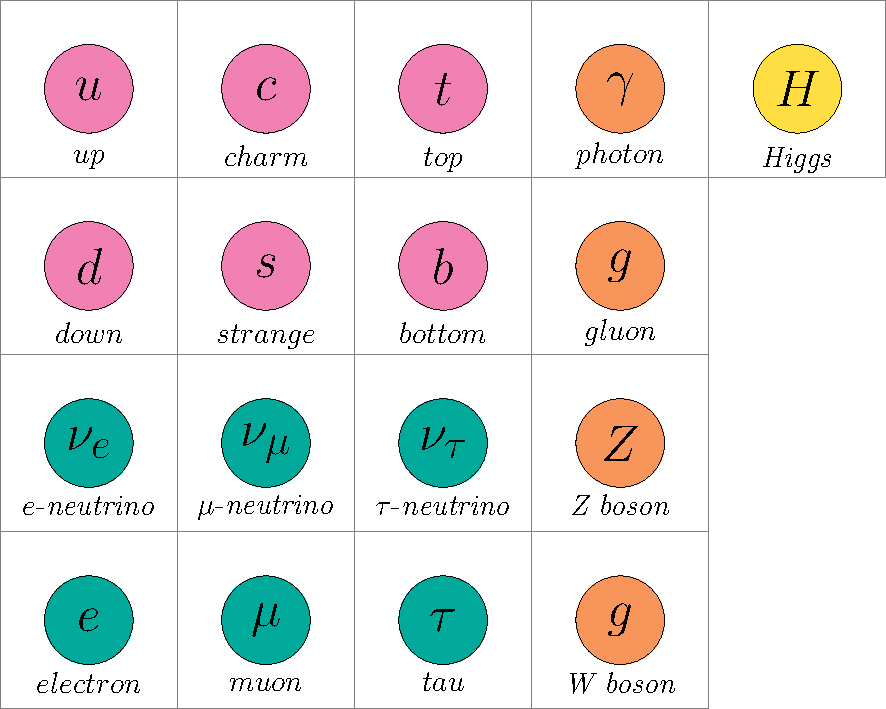
\includegraphics[width=7cm]{Images/SM-particles.pdf}
\caption[Campos cuánticos del Modelo Estándar]{El ME explica cómo los componentes básicos de la materia (los quarks y los leptones) interactúan a través de tres de las cuatro fuerzas fundamentales.}
\label{SMparticles}
\end{figure}


\section[\hspace{-0.175in} El sector electrodébil]{El sector electrodébil}

Las partículas del ME ganan masa por medio del mecanismo de Higgs, el cual es una realización de la quiebra espontánea de la simetría, $SU(2)_L \times U(1)_Y \rightarrow U(1)_Q$, donde $Q$ es la carga eléctrica. En la tabla \ref{table1} podemos ver los números cuánticos del contenido de matéria del ME donde $I$ es el isospín débil e $I_3$ es su tercera componente. La carga eléctrica se calcula a partir de la relación Gell-Mann$-$Nishijima $Q=I_3 + Y/2$. 


\begin{table}[h]
\caption[\hspace{-0.15in}Números cuánticos del Modelo Estándar]{Números cuánticos electrodébiles de los fermiones en el modelo estándar. Las tres generaciones de los quarks y los letones están representadas por un solo símbolo $Q$ y $L$ para los dobletes de $SU(2)_L$ y $q_R,\ell_R$ para los singletos. Los subíndices $L$ y $R$ denotan quiralidad izquierda y derecha, respectivamente.}
\begin{center}
\begin{small}
\begin{tabular}{|c | c | c | c | c|} 
 \hline
 Representaciones irreducibles & & & & \\ fermiónicas de $SU(2)_L \times U(1)_Y$ & $I$ & $I_3$ & $Y$ & $Q$ \\ [1ex] 
 \hline\hline
 $L \equiv 
	\begin{pmatrix}
	\nu \\
	\ell 
	\end{pmatrix}_L $ & $1/2$ & $\begin{array}{c} 1/2 \\ \hspace{-0.1in} -1/2 \end{array}$	 & \hspace{-0.1in} $-1$ & $0$ \\ 
[1ex]
 \hline
 $\ell_R$ & $0$ & $0$ & \hspace{-0.1in} $-2$ & $1$ \\ [0.25ex] 
 \hline
  $Q \equiv 
	\begin{pmatrix}
	u \\
	d 
	\end{pmatrix}_L $ & $1/2$ & $\begin{array}{c} 1/2 \\ \hspace{-0.1in} -1/2 \end{array}$	 & $1/3$ & $\begin{array}{c} 2/3 \\ \hspace{-0.1in} -1/3 \end{array}$ \\ 
[1ex]
 \hline
  $u_R$ & $0$ & $0$ & $4/3$ & $2/3$ \\ [0.25ex] 
 \hline
 $d_R$ & $0$ & $0$ & \hspace{-0.1in} $-2/3$ & \hspace{-0.1in} $ -1/3$ \\ [0.25ex] 
 \hline
\end{tabular}
\end{small}
\label{table1}
\end{center}
\end{table}


Con la simetría gauge del ME y el contenido de matéria verificado experimentalmente podemos construir la lagrangeana del sector electrodébil,
\begin{eqnarray}
\mathcal{L} &=& i \overline{L} \slashed{D} L + i \overline{Q} \slashed{D} Q + i \overline{\ell_R} \slashed{D} \ell_R +  i \overline{u_R} \slashed{D} u_R + i \overline{d_R} \slashed{D} d_R  \nonumber \\
            &-& \frac{1}{4} \vec{F}^{\mu \nu} \cdot \vec{F}_{\mu \nu} -\frac{1}{4}B_{\mu \nu} B^{\mu \nu} \nonumber \\
             &+&\left(D_\rho \Phi \right)^\dagger \left( D^\rho \Phi \right) + \mu^2 \Phi^\dagger \Phi - \lambda \left( \Phi^\dagger \Phi \right)^2 \nonumber \\
             &-& \left[ Y^{\ell}\, \overline{L}\Phi \ell + Y^{u}\, \overline{Q}(-i\sigma_2 \Phi^*) u + Y^{d}\, \overline{Q}\Phi d  + H.c.  \right],
\end{eqnarray}
donde la derivada covariante es $D_\mu \equiv \partial_\mu + ig\vec{A}_\mu \cdot\vec{\sigma}/2 +ig' B_\mu Y/2$ y tanto $\vec{A}_\mu$ como $B_\mu$ son bosones de gauge de los grupos $SU(2)_L$ y $U(1)_Y$, respectivamente, $\sigma_2$ es la segunda matriz de Pauli y $\Phi$ es el doblete de Higgs cuyos números cuánticos son mostrados en la tabla \ref{table2}

\begin{table}[h]
\caption{\hspace{-0.15in}Números cuánticos electrodébiles para el doblete de Higgs.}
\begin{center}
\begin{small}
\begin{tabular}{|c | c | c | c | c|} 
 \hline
Doblete de Higgs & $I$ & $I_3$ & $Y$ & $Q$ \\ [1ex] 
 \hline\hline
 $\Phi \equiv 
	\begin{pmatrix}
	\phi^+ \\
	\phi^0 
	\end{pmatrix} $ & $1/2$ & $\begin{array}{c} 1/2 \\ \hspace{-0.1in} -1/2 \end{array}$	 & $1$ & $\begin{array}{c} 1 \\ 0 \end{array}$ \\ 
[1ex]
 \hline
\end{tabular}
\end{small}
\label{table2}
\end{center}
\end{table}

 Cabe notar que los neutrinos no son las únicas partículas del ME que permanecen sin masa después del rompimiento espontáneo de simetría. Los fotones y los gluones también permanecen no masivos, pero a diferencia de los neutrinos, esto se debe a que $SU(3)_C \times U(1)_Q$ permanece como una simetría del ME después de la quiebra de simetría. Este mistério  relacionado al origen de las masas de los neutrinos es física está más allá del ME es una de las áreas de investigación más activas actualmente.



\section[\hspace{-0.19in} Tests del modelo estándar]{Tests del modelo estándar}

A lo largo de su história, el modelo estándar ha probado que funciona muy bien al superar varias pruebas. En esta sección comentaremos un poco sobre algunos de esos tests, básicamente aquellos que fueron hechos en el CERN\footnote{Conseil Européen pour la Recherche nucléaire $-$ Consejo Europeo para la Investigación Nuclear.}.

El gran colisionador de electrones y positrones LEP\footnote{Large Electron-Positron collider \href{https://home.cern/science/accelerators/large-electron-positron-collider}{LEP}.} en el CERN operó de 1989 al 2000. Este acelerador circular contaba con un anillo de aproximadamenteo 27 km y habían cuatro detectores multipropósito: L3, ALEPH, OPAL y DELPHI (ver figura \ref{LEPmap}).

\begin{figure}[h]
\centering
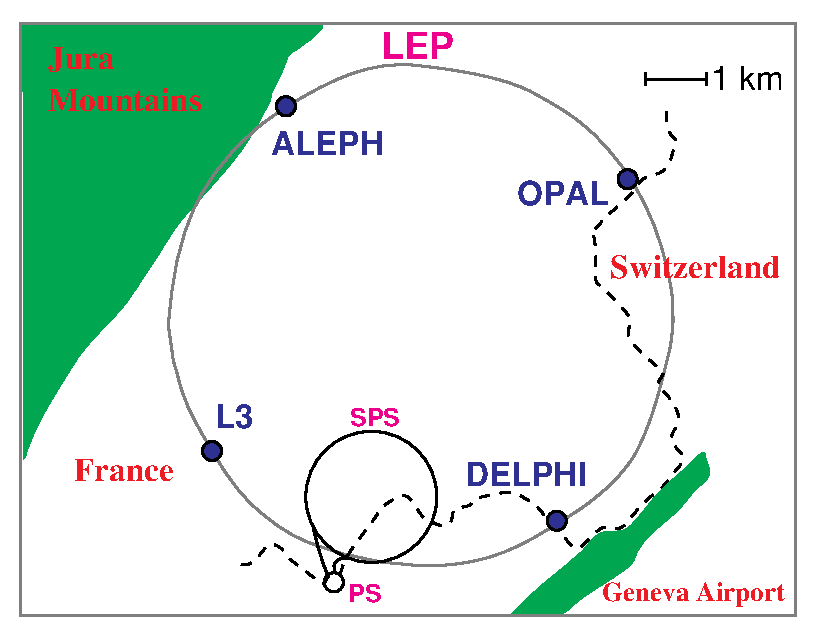
\includegraphics[scale=0.8]{Images/lep_map.eps}
\caption[Mapa del Large Electron-Positron Collider (LEP)]{Mapa del Large Electron-Positron Collider (LEP) \cite{aleph2005precision}.}
\label{LEPmap}
\end{figure}

Al final de la toma de datos con energias del centro de masa alrededor de la resonancia del bosón Z, cerca de 1000 bosones Z eran registrados cada hora por cada uno de los cuatro experimentos previamente mencionados. Esto hizo de LEP una fábrica de bosones Z y algunos de sus resultados fueron:
\begin{itemize}
	\item \textbf{La resonancia del bosón Z:} La sección de choque de la colisión $e^+e^-$ sufre un incremento de cerca de 3 ordenes de magnitud cuando la energía del centro de masa alcanza la masa del bosón Z, $m_Z$. Esto se debe a que el bosón Z acopla con todos los fermiones de manera similar a los fotones. Aparece entonces un competidor para este último al momento de mediar dicha interacción. Para energías abajo de $\sim 40$ GeV, el fotón domina. A energías mayores ambos son igual de importanes, pero cerca de la resonancia del bosón Z, este domina. Esto se entiende en el ME debido a que la amplitud total del proceso es $\mathcal{M}=\mathcal{M}_\gamma+\mathcal{M}_Z$, $\mathcal{M}_\gamma\propto 1/q^2 $, $\mathcal{M}_Z \propto 1/[q^2 -m_Z^2 + im_Z\Gamma_Z]$, $\Gamma_Z$ es el ancho de decaimiento del bosón Z, siendo la sección total de choque es proporcional a $|\mathcal{M}|^2=|\mathcal{M}_\gamma+\mathcal{M}_Z|^2$. De esta manera, cada mediador tiene su región donde domina pero también existen regiones donde interfieren y ninguno lo hace (ver la figura \ref{SMt1}).
	
	
\begin{figure}[h!]
\centering
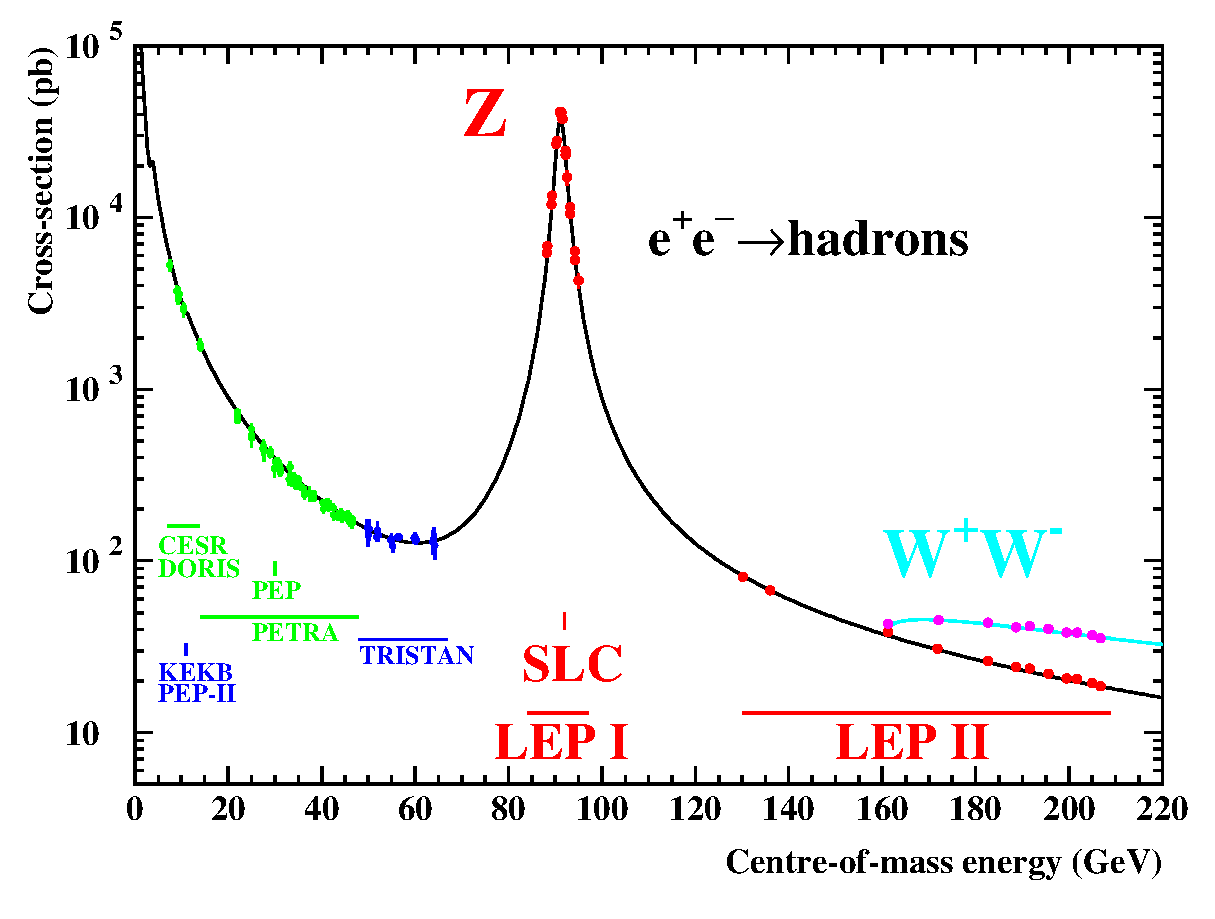
\includegraphics[scale=0.55]{Images/SM-test-1.eps}
\caption[Sección de choque hadrónica en la resonancia del boson Z]{Sección de choque hadrónica en la resonancia del boson Z \cite{aleph2005precision}. El pico en la sección de choque para $e^+e^-\to$ hadrons cerca de $\sim$90 GeV no se puede explicar con la electrodinámica cuántica (QED). El bosón Z del ME puede explicar este aumento.}
\label{SMt1}
\end{figure}
	
\newpage	
	\item \textbf{El ancho de decaimiento del bosón Z:} Aunque los neutrinos no sean observados en los experimentos previamente mencionados, ellos afectan significativamente el ancho de decaimiento del bosón Z, esto es \cite{thomson2013modern}
	\begin{equation}
	\Gamma_Z = 3\Gamma_{\ell \ell} + \Gamma_{\rm hadrons} + n_\nu\Gamma_{\nu\nu},
	\end{equation}	  
	asumiendo universalidad leptónica\footnote{Esto quiere decir que las diferentes generaciones de leptones acoplan de la misma manera con los bosones de gauge.}. 
	
En la figura \ref{SMt2} se muestra que $n_\nu =3$ da el mejor ajuste a los datos combinados de los cuatro experimentos. Este resultado está de acuerdo con otros resultados experimentales independientes como, por ejemplo, el número efectivo de neutrinos $N_{\rm eff}=2.99(17)$ obtenidos del estudio del fondo cósmico de microondas (CMB)\footnote{Ver el siguiente capítulo.} hecho por la colaboración Planck \cite{aghanim2020planck}. Sin embargo, podría existir otros `neutrinos' más pesados que no pueden ser producidos en los decaimientos del bosón Z y no afectan el número de especies relativísticas del universo en el momento de la formación del CMB.
	
\begin{figure}[h!]
\centering
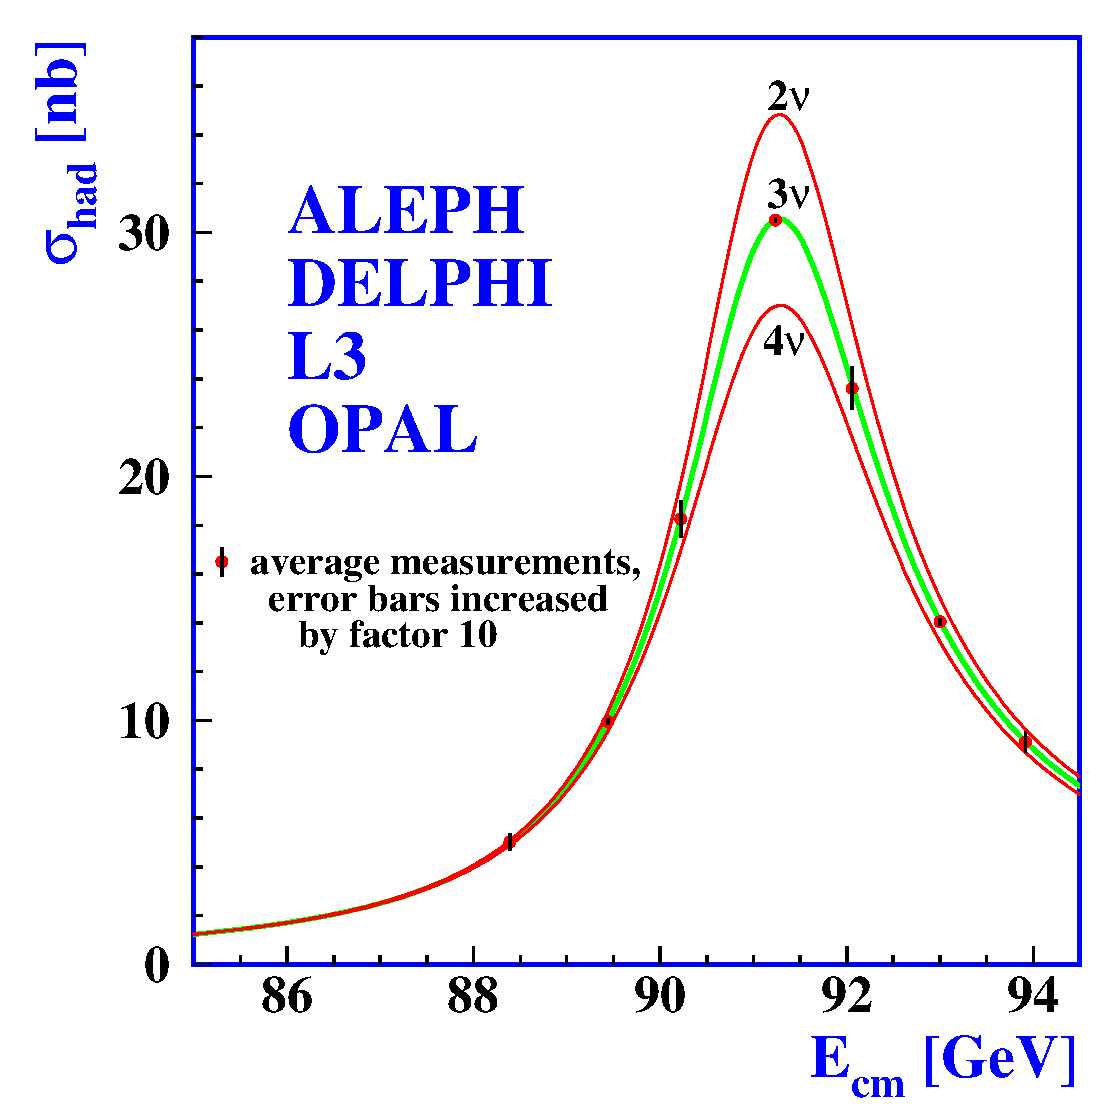
\includegraphics[scale=0.55]{Images/SM-test-2.eps}
  \caption[Sección de choque variando con el número de neutrinos]{Sección de choque variando con el número de neutrinos \cite{aleph2005precision}. Mediciones del ancho de decaimiento del bosón Z concuerdan con la predicción del ME cuando el número de neutrinos activos es 3. Actualmente no se han observado más de tres de estos neutrinos ni sus respectivos leptones a los que asociados.}
  \label{SMt2}
\end{figure}
	
	
\newpage	
	
\item \textbf{Masa de los bosones W:} En LEP, a diferencia del bosón Z, la masas de los bosones W son obtenidas de la producción de pares $W^+W^-$. Cerca de $\sqrt{s}=2\,m_W$, la sección de choque $\sigma (e^+e^- \to W^+W^-)$ depende fuertemente de $m_W$ y $\Gamma_W$ ya que los W están \textit{on-shell}\footnote{Esto quiere decir que cumplen $E^2=m^2+p^2$.}, pero para energías del centro de masa $\sqrt{s}$ mayores, se debe reconstruir las masas invariantes de los productos finales considerando a los bosones $W$ tanto \textit{on-shell} como virtuales (ver figura \ref{eeWW}).
\begin{figure}[h]
\centering
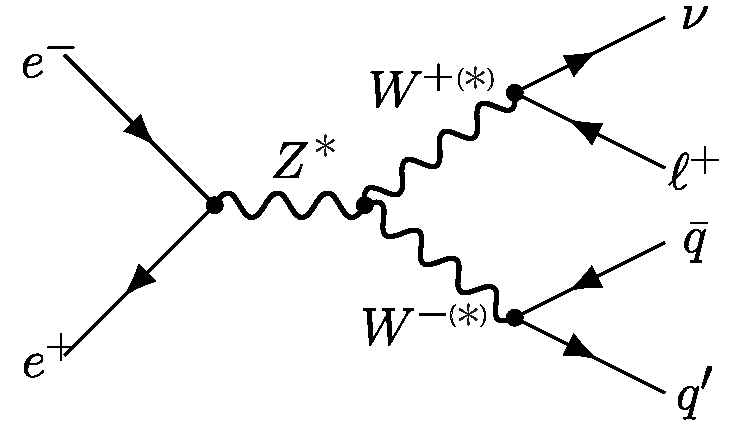
\includegraphics[scale=0.45]{Images/ee_to_WW.pdf}
\caption[Diagrama de Feynman para $e^+e^- \to W^+W^-$ con estado final $qq\ell \nu$]{Diagrama de Feynman para $e^+e^- \to W^+W^-$ con estado final de tipo $qq\ell \nu$. La colaboración L3 analizó estados finales conteniendo cuatro fermiones: $\ell \nu\ell \nu$, $qq\ell \nu$ y $qqqq$.}
\label{eeWW}
\end{figure}

%La colaboración L3 analizó estados finales conteniendo cuatro fermiones: $\ell \nu\ell \nu$, $qq\ell \nu$ y $qqqq$. En la figura \ref{eeWW} podemos ver el diagrama de Feynman para un proceso donde las masas invariantes $m_1^2=(p_\nu + p_\ell)^2$ y $m_2^2=(p_{\bar{q}}+p_q)^2$ son diferentes. 


\  \

En la figura \ref{SMt3} podemos ver esta sección de choque $\sigma (e^+e^- \to W^+W^-)$ medida a $\sqrt{s}=$ 161 GeV \cite{acciarri1997pair}, 172 GeV \cite{acciarri1997measurement}, 183 GeV \cite{acciarri1998measurement} y valores mayores \cite{achard2004measurement}. Cuando los bosones $W$ son virtuales, sus masas mudan en cada evento y son, en general, distintas entre sí. La figura \ref{SMt4} muestra la distribución del promedio de estas masas para los eventos $e^+e^- \to W^{+}W^{-}\to q\bar{q}\ell \nu$. Los resultados de las simulaciones Monte Carlo del ME están muy de acuerdo con estos dos resultados experimentales\footnote{Recientemente la colaboración CDF anunció una medida de la masa del W que discrepa con la predicción del ME \cite{cdf2022high}. Este resultado se aleja de los valores reportados por otros experimentos los cuales también son muy precisos y están de acuerdo con el ME.}. 
\end{itemize}


\begin{figure}[h!]
\centering
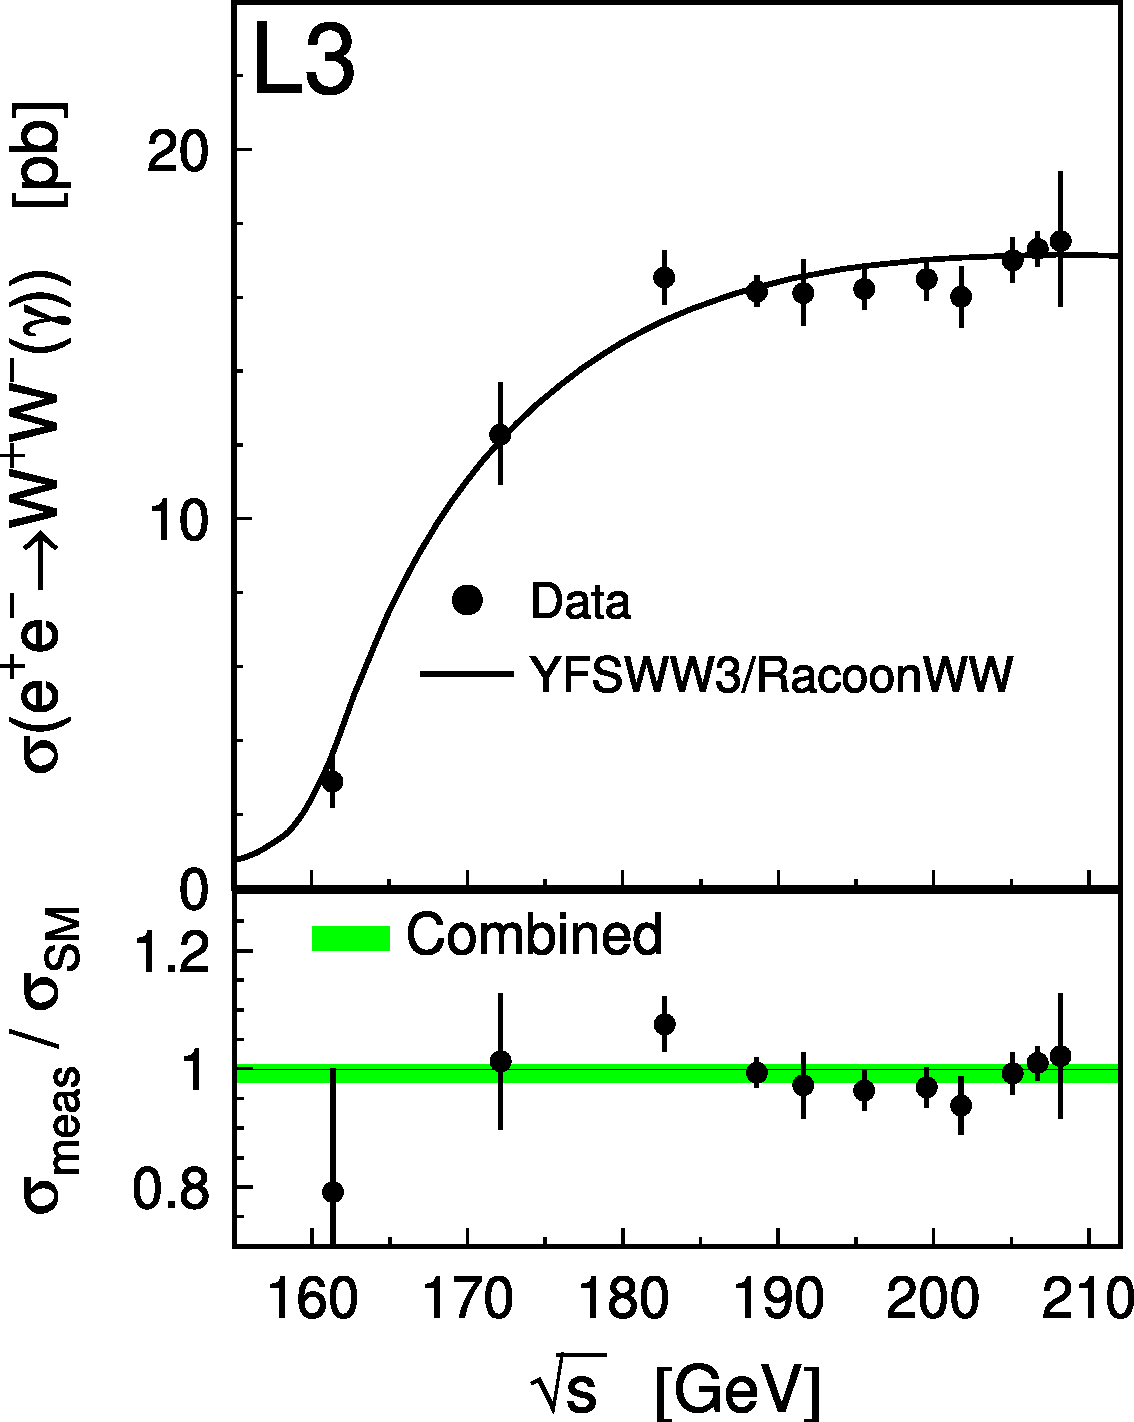
\includegraphics[scale=0.35]{Images/SM-test-6.pdf}
\caption[Sección de choque de $e^+e^- \to W^+W^-$]{Sección de choque de $e^+e^- \to W^+W^-$ \cite{achard2004measurement}. Los resultados experimentales para la sección de choque para $e^+e^- \to W^+W^-$ concuerdan con la predicción del ME.}
\label{SMt3}
\end{figure}

\begin{figure}[h!]
\centering
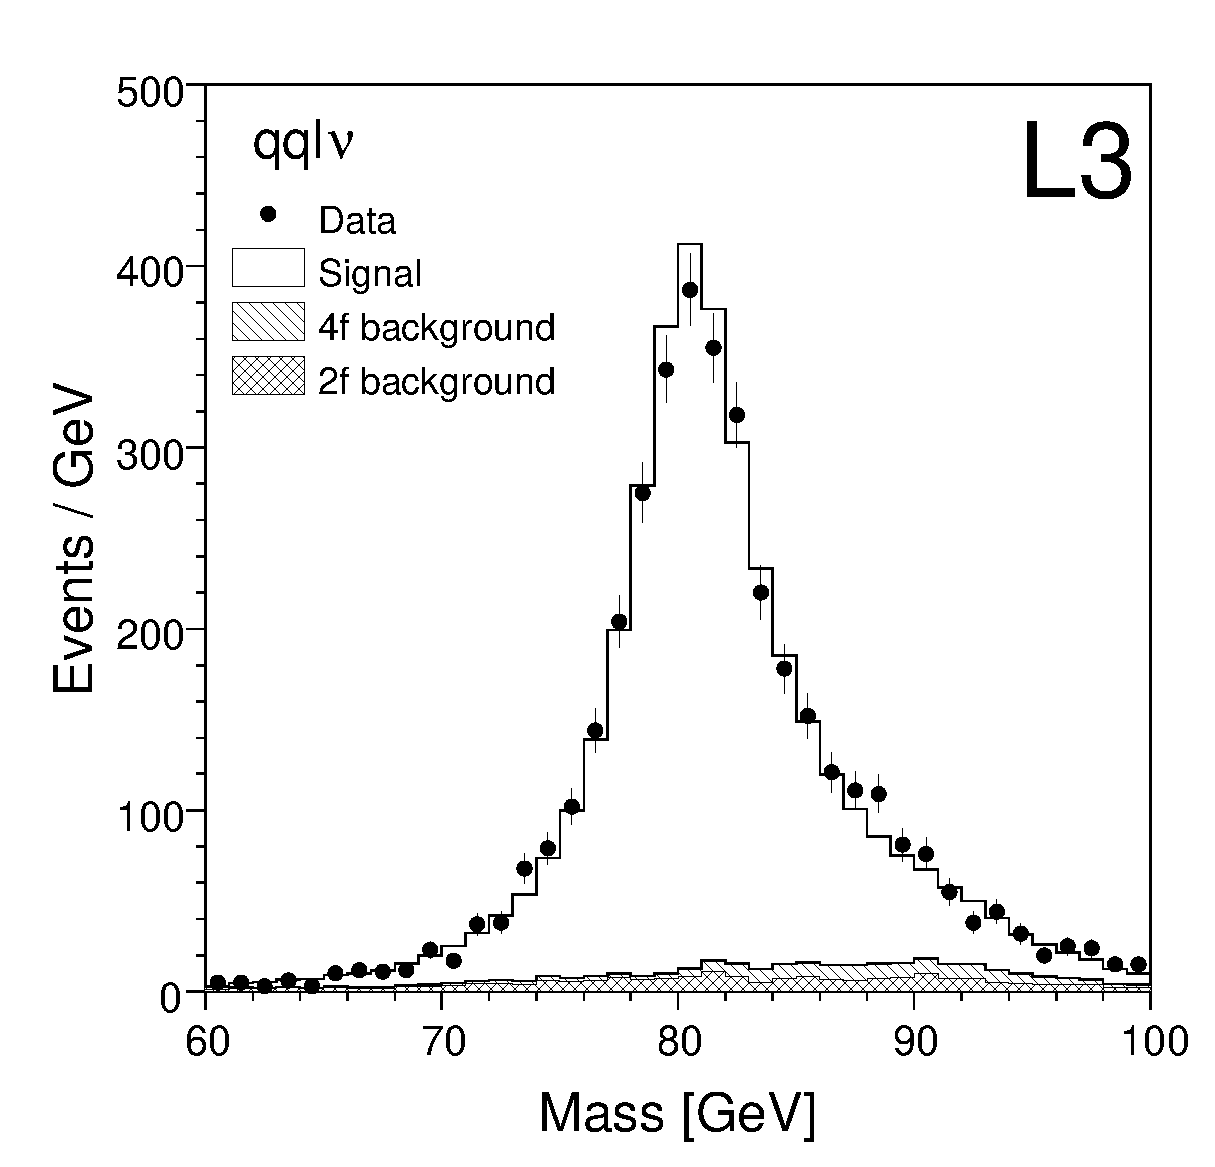
\includegraphics[scale=0.4]{Images/SM-test-3.eps}
\caption[Distribución de masas reconstruidas del bosón W]{Distribución de masas reconstruidas del bosón W \cite{l32006measurement}. La distribución de la masa del W concuerda con las simulaciones Monte Carlo en el contexto del ME.}
 \label{SMt4}
\end{figure}



\begin{itemize}
	\item \textbf{Asimetría forward-backward:} Los productos de la colisión $e^+e^-$ mediados por un bosón Z (por ejemplo, $e^+e^- \to Z^* \to \mu^+\mu^-$, ver figura \ref{eeZmumu}) aparecen haciendo un ángulo $\theta$ con relación al eje de los haces iniciales. 
\begin{figure}[h]
\centering
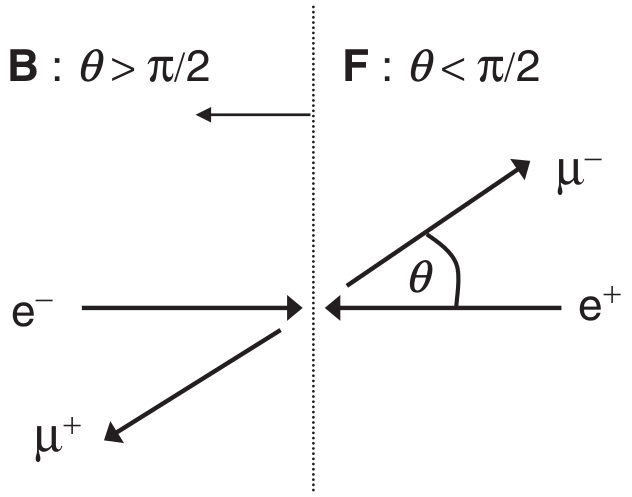
\includegraphics[scale=0.2]{Images/A_FB.png}
\caption[Par $\mu^+\mu^-$ producido en la colisión $e^+e^-$]{Par $\mu^+\mu^-$ producido en la colisión $e^+e^-$ \cite{thomson2013modern}.}
\label{eeZmumu}
\end{figure}	
	
	Esta distribución no es isotrópica en el ME ya que los acoplamientos del bosón Z con fermiones de mano derecha e izquierda son diferentes. Por ejemplo, para el proceso $e^+e^- \to Z^* \to \mu^+\mu^-$ tenemos (ignorando contribuciones de la QED cerca de $\sqrt{s}\sim m_Z$),
\[
\mathcal{M} = - \frac{g_z^2}{s-m_Z^2+i m_Z \Gamma_Z} g_{\mu \nu}\bigg[ \bar{v} \gamma^\mu \frac{1}{2} \left( c_V^e -c_A^e \gamma^5 \right) u \bigg] \bigg[ \bar{u} \gamma^\mu \frac{1}{2} \left( c_V^\mu -c_A^\mu \gamma^5 \right) v \bigg]
\]
y de ahí se obtiene
\begin{equation}
\frac{d\sigma}{d\Omega} \propto  a (1+\cos^2\theta) + 2b \cos \theta 
\end{equation}
donde
\begin{equation}
a = \left[ (c^e_L)^2+(c^e_R)^2 \right]\left[ (c^\mu_L)^2+(c^\mu_R)^2 \right], \hspace{0.05in} b = \left[ (c^e_L)^2-(c^e_R)^2 \right]\left[ (c^\mu_L)^2-(c^\mu_R)^2 \right]
\end{equation}

Esta asimetría $A_{\rm FB}$ se mide calculando las secciones de choque \textit{forward} $\sigma_F$ y  \textit{backward} $\sigma_B$,
\begin{equation}
\sigma_F \equiv 2 \pi \int_0^1 \frac{d\sigma}{d \Omega} d(\cos \theta ), \hspace{0.25in} \sigma_B \equiv 2 \pi \int_{-1}^0 \frac{d\sigma}{d \Omega} d(\cos \theta ),
\end{equation}
de manera que
\begin{equation}
A_{\rm FB} \equiv \frac{\sigma_F - \sigma_B}{\sigma_F + \sigma_B}.
\end{equation}

En la figura \ref{SMt5} se muestra evidencia experimental de esta asimetría en la sección diferencial de choque en función de $\cos \theta$ para $e^+e^- \to Z^* \to \mu^+ \mu^-$ justo como dice el ME.

Si el bosón Z acoplase de la misma manera con fermiones de mano derecha y de mano izquierda, entonces tendríamos $b=0$ y la distribución angular sería simétrica $(1+\cos^2\theta)$ dando como resultado $A_{\rm FB} = 0$.


\end{itemize}



\begin{figure}[h!]
\centering
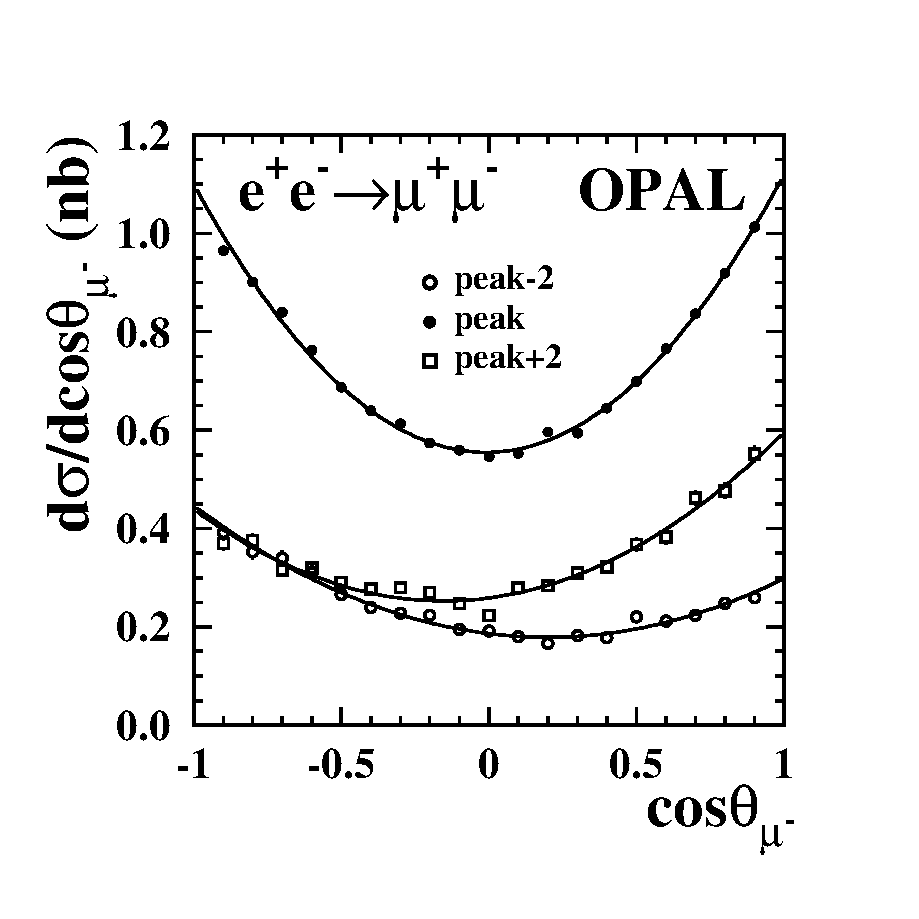
\includegraphics[scale=0.5]{Images/SM-test-5.eps}
  \caption[Asimetría forward-backward]{La asimetría \textit{forward-backward} a pesar de ser pequeña es claramente un indicador de que el bosón Z acopla diferente con los fermiones de mano derecha e izquierda. $A_{\rm FB}=0$ para procesos mediados puramente por QED  \cite{opal2001precise}.}
 \label{SMt5}
\end{figure}



\section[\hspace{-0.19in} Física del Higgs]{Física del Higgs}

%\color{red}
%(to be completed): read Maggiore.
%\color{black}


Descubierto en 2012 por las colaboraciones ATLAS \cite{ATLAS:2012yve} y CMS \cite{CMS:2012qbp}, el bosón de Higgs es la pieza final del modelo estándar. Esta partícula es especial en el sentido de que es la única partícula fundamental con spin cero que conocemos. Sus decaimientos han sido estudiados ampliamente; sin embargo, poco se sabe de su acople trilinear y además hay indicios de que podría haber otros escalares neutros más ligeros \cite{CMS:2018cyk,CMS:2023yay,CMS:2024yhz} o más pesados \cite{Kundu:2024sip} que estarian al alcance de próximos experimentos.

Se conocerá más sobre el Higgs, por ejemplo, en futuros colisionadores de muones ya que tienen la ventaja de ser de precisión como los colisionadores de $e^+e^-$ y llegarían a altas energías comparables a la de los del gran colisionador hadrónico \footnote{Un colisionador de muones a energía de centro de masa de 10 TeV es comparable con el LHC a 100 TeV \url{https://home.cern/science/accelerators/muon-collider}.}.


\section[\hspace{-0.2in} Conclusiones]{Conclusiones}

El modelo estándar ha probado ser un gran logro de la ciencia moderna. En este capítulo, hemos visto como ha superado varios tests en colisionadores, lo cual justifica su nombre. Sin embargo, el no incluir a, por ejemplo, la interacción gravitacional, es una señal de que debemos ir más allá de este modelo.
%\color{red}
%conclusiones de este capítulo: El ME es genial, funciona muy bien, pero todavia necesitamos más experimentos. Futuros experimentos como el colisionador de muones podrán testar triple vertex (limites superiores aún son muy débiles )
%\color{black}














